

%----------------------------------------------------------------------------------------
%	PACKAGES AND OTHER DOCUMENT CONFIGURATIONS
%----------------------------------------------------------------------------------------

\documentclass[12pt]{article}

\usepackage{polski}
\usepackage[polish]{babel}
\usepackage[utf8]{inputenc}
\usepackage{datetime}
\usepackage{graphicx}
\usepackage{tikz}
\usepackage{amsmath}
\usepackage{epstopdf}
\usepackage{multirow}
\usepackage{tabularx}
%\usepackage[colorlinks=true]{hyperref}
%\usepackage[all]{hypcap}
%\usepackage{showframe} 
\usepackage{geometry}
 \geometry{
 a4paper, 
 left=20mm,
 right=20mm,
 top=20mm,
 bottom=20mm,
 }
 
%----------------------------------------------------------------------------------------
 
%----------------------------------------------------------------------------------------
% DATES
%----------------------------------------------------------------------------------------

\renewcommand{\dateseparator}{.} 
\newdate{exercise_date}{04}{06}{2014}

%----------------------------------------------------------------------------------------

%----------------------------------------------------------------------------------------
% TIKZ PACKAGES
%----------------------------------------------------------------------------------------

\usetikzlibrary{arrows}

%----------------------------------------------------------------------------------------

\begin{document}
 
\begin{titlepage}

\newcommand{\HRule}{\rule{\linewidth}{0.5mm}}
% Defines a new command for the horizontal lines, change thickness here

\center
% Center everything on the page
 
%----------------------------------------------------------------------------------------
%	LOGO SECTION
%----------------------------------------------------------------------------------------

\includegraphics[width=6cm]{../res/img/logo.png}\\[1cm]
% Include a department/university logo - this will require the graphicx package
 
%----------------------------------------------------------------------------------------
 
%----------------------------------------------------------------------------------------
%	HEADING SECTIONS
%----------------------------------------------------------------------------------------

\textsc{\LARGE Akademia Górniczo-Hutnicza \\[0.2cm]
im. Stanisława Staszica w Krakowie}\\[1.5cm]
% Name of your university/college

\textrm{\Large Wydział Elektrotechniki Automatyki Informatyki i Inżynierii
Biomedycznej}\\[1cm]

\textsc{\Large Laboratorium Aparatury Automatyzacji}\\[0.5cm]
% Major heading such as course name

%----------------------------------------------------------------------------------------
%	TITLE SECTION
%----------------------------------------------------------------------------------------

\HRule \\[0.4cm]
{ \huge \bfseries Prosty regulator mikroprocesorowy 
}\\%[0.4cm]
% Title of your document
\HRule \\[1.5cm]

%----------------------------------------------------------------------------------------
%	REPORT TABLE
%----------------------------------------------------------------------------------------

\begin{table}[h]
\centering
\begin{tabularx}{\linewidth}{|c|l|X|}
\hline
% \multicolumn{3}{|c|}{
% \begin{tabular}{cc}
% \begin{tabular}{c}
% \includegraphics[height=2.2cm]{../res/img/logo.jpg}\\
% \end{tabular}
% &
% \begin{tabular}{c}
% \Large{Akademia Górniczo-Hutnicza im. Stanisława Staszica}\\[5pt]
% \large{\textsc{Katedra Automatyki}}\\[5pt]
% \textsc{Laboratorium Aparatury Automatyzacji}
% \end{tabular}
% \end{tabular}
% }\\
% \hline
% \multicolumn{3}{|c|}{}\\[-5pt]
% \multicolumn{3}{|c|}{\textbf{\huge{Ćwiczenie 6}}}\\[10pt]
% \multicolumn{3}{|c|}{\Large{Bezpośrednie sterowanie cyfrowe}}\\[8pt]
% \hline
\multicolumn{2}{|c|}{Wydział EAIiIB, kierunek AiR, rok II}
& Grupa 6, wtorek 11:00-12:30\\
\hline
Lp. & Imię i nazwisko & Zaliczenie\\
\hline
1 & \textbf{Konrad Adasiewicz} & \\
\hline
2 & \textbf{Michał Maciejewski} & \\
\hline
3 & \textbf{Bartosz Szmit} & \\
\hline
\multicolumn{2}{|c|}{Data wykonania ćwiczenia:
\ddmmyyyydate\displaydate{exercise_date}r.} & Data oddania sprawozdania:
\ddmmyyyydate\displaydate{create_date}r.
\\
\hline
\end{tabularx}
\end{table}

%----------------------------------------------------------------------------------------

\vfill % Fill the rest of the page with whitespace

\end{titlepage} 

% \section{Wstęp}
% 
% 
% 
% 
% 
% \subsubsection{Analiza serwomechanizmu przekaźnikowego z wykorzystaniem
% płaszczyzny fazowej}
% \subsection{Cel ćwiczenia}
% Celem ćwiczenia jest zapoznanie się z zastosowaniem metody płaszczyzny fazowej do analizy nieliniowych 
% układów regulacji na przykładzie serwomechanizmu przekaźnikowego. Podczas ćwiczenia zbadany zostanie 
% wpływ parametrów zarówno przekaźnika, jak i obiektu na przebieg trajektorii fazowych serwomechanizmu 
% przy zerowym wymuszeniu i starcie z niezerowych warunków początkowych. Należy zbadać przebieg 
% trajektorii fazowych dla układu regulacji złożonego z obiektu o transmitancji: 
% 
% \begin{equation*}
% 	G(s)=\frac{K}{s(Ts+1)}
% \end{equation*}
% 
% oraz regulatora III położeniowego z histerezą przy starcie z różnych warunków
% początkowych i zerowym wymuszeniu.
% 
% \newpage

\section{Dyskretne układy regulacji}

\subsection{Cel ćwiczenia}

Celem ćwiczenia jest zapoznanie się z podstawowymi własnościami układów regulacji składających się z 
ciągłego obiektu regulacji sterowanego regulatorem dyskretnym. Charakterystyczną cechą systemów 
dyskretnych jest zależność własności układu, np. stabilności, nie tylko od
parametrów obiektu i nastaw regulatora, lecz także od okresu próbkowania. Podczas ćwiczenia zostanie zbadany wpływ okresu próbkowania 
na stabilność dyskretnego układu regulacji. Zostanie rozważony zamknięty układ regulacji złożony z 
dyskretnego regulatora typu P (proporcjonalnego) oraz obiektu inercyjnego: I rzędu (część 1 ćwiczenia) oraz 
III rzędu (część 2 ćwiczenia). Okazuje się, że w układach dyskretnych możliwa jest utrata stabilności nawet w 
przypadku obiektu I rzędu sterowanego regulatorem proporcjonalnym, co w przypadku układów ciągłych jest 
niemożliwe.

\subsection{Obiekt pierwszego rzędu}

Poniżej zamieszczam schemat zastępczy układu regulacji cyfrowej obiektu
pierwszego rzędu:

\begin{figure}[!htb]
	\begin{center}
		\includegraphics[width=14cm]{../res/img/schd1.png} 
	\end{center}
	\caption{Schemat badanego układu z obiektem inercyjnym pierwszego rzędu}
\end{figure}

Dla tak zestawionego układu wyznaczyliśmy odpowiedzi skokowe i przebiegi
sterowania dla wzmocnienia krytycznego przy poszczególnych okresów próbkowania,
$Tp\in \{0.01, 0.1, 1, 5, 10\}[s]$. Poniżej zamieszczone owe odpowiedzi z
krótkimi opisami parametrów dla których zostały ściągnięte.

\newpage

\begin{figure}[!htb]
	\begin{center}
		\includegraphics[trim=5cm 9cm 5cm 9cm,width=10cm]{../res/img/d1_0,01_1000y.pdf} 
	\end{center}
	
	\begin{center}
		\includegraphics[trim=5cm 9cm 5cm 9cm,width=10cm]{../res/img/d1_0,01_1000u.pdf} 
	\end{center}
	\caption{Odpowiedź obiektu 1-wszego rzędu dla parametrów $k=1000$,
	$T_p=0,01[s]$}
\end{figure}

\newpage

\begin{figure}[!htb]
	\begin{center}
		\includegraphics[trim=5cm 9cm 5cm 9cm,width=10cm]{../res/img/d1_0,1_100y.pdf} 
	\end{center}
	
	\begin{center}
		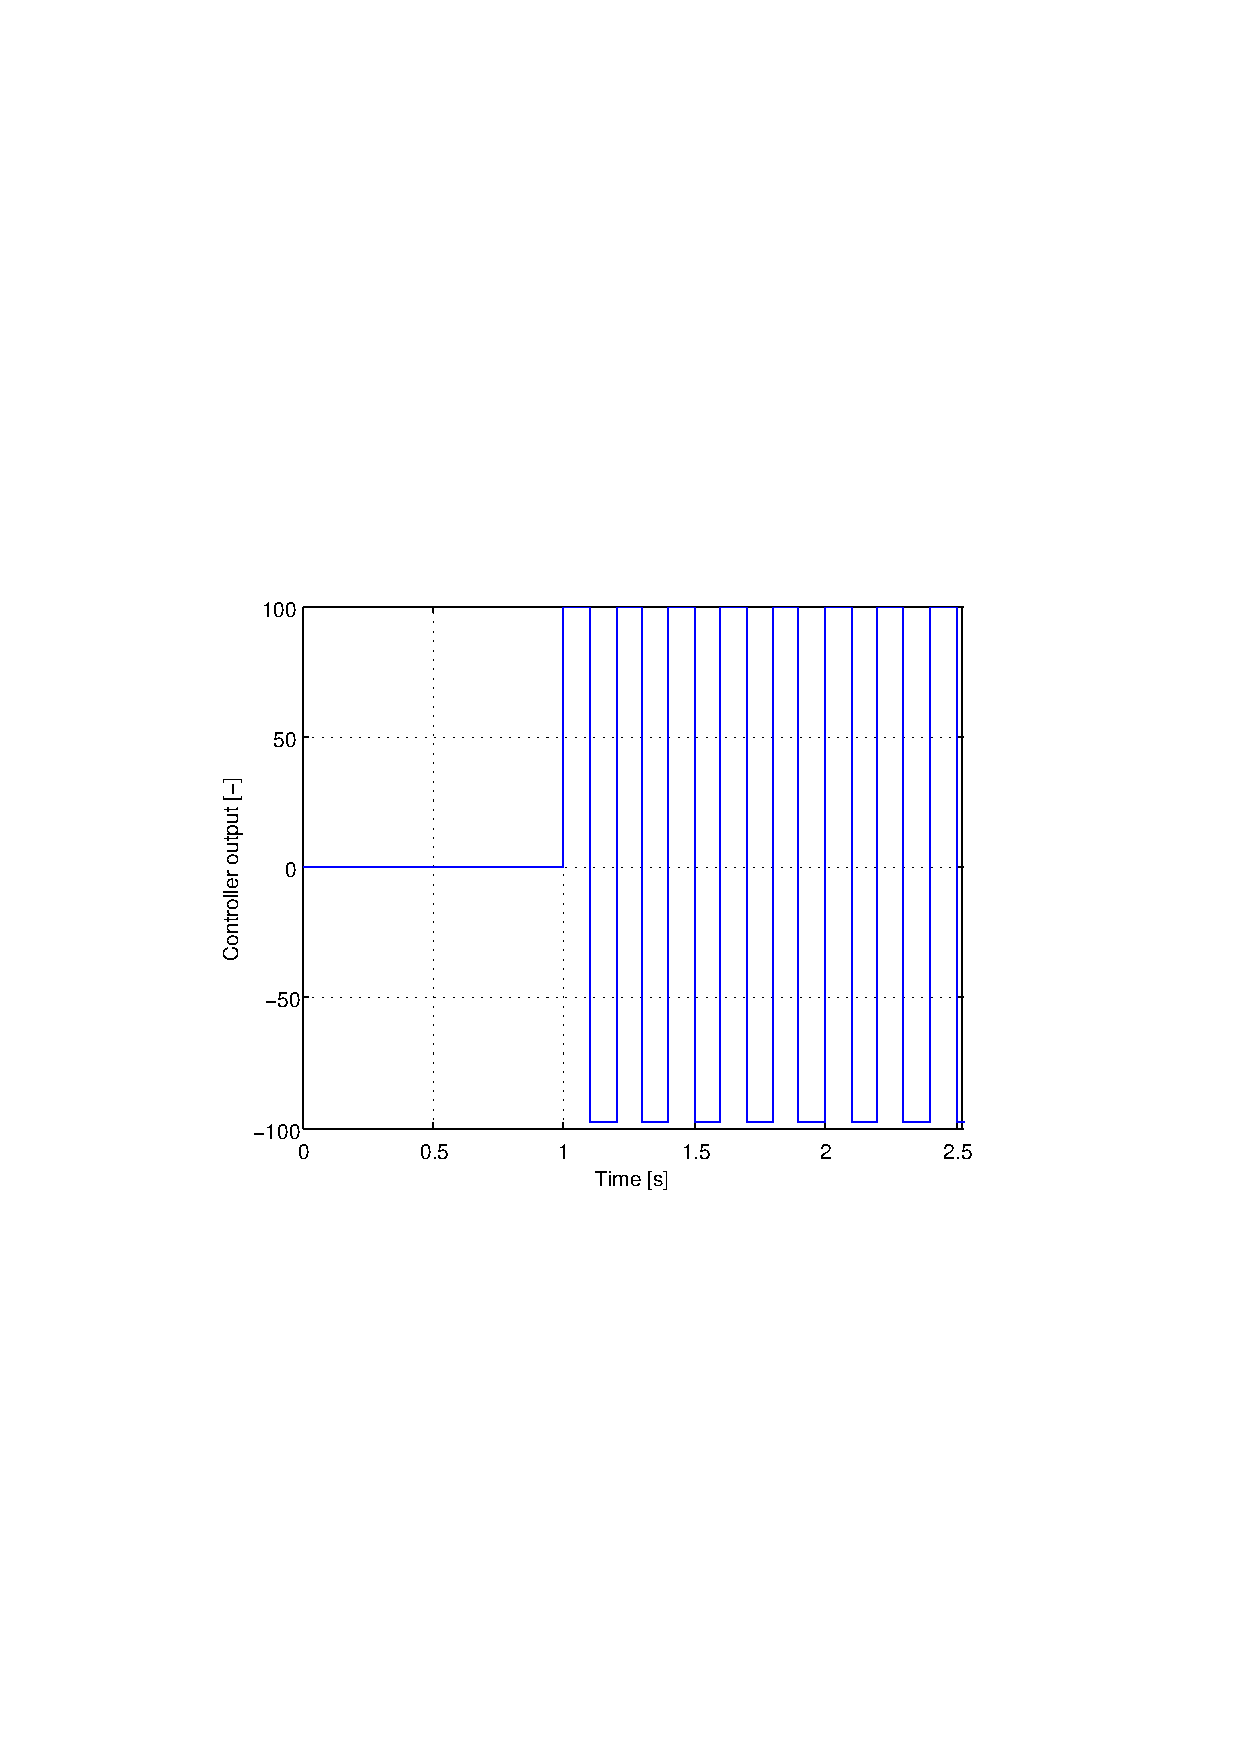
\includegraphics[trim=5cm 9cm 5cm 9cm,width=10cm]{../res/img/d1_0,1_100u.pdf} 
	\end{center}
	\caption{Odpowiedź obiektu 1-wszego rzędu dla parametrów $k=100$,
	$T_p=0,1[s]$}
\end{figure}

\newpage

\begin{figure}[!htb]
	\begin{center}
		\includegraphics[trim=5cm 9cm 5cm 9cm,width=10cm]{../res/img/d1_1_10y.pdf} 
	\end{center}
	
	\begin{center}
		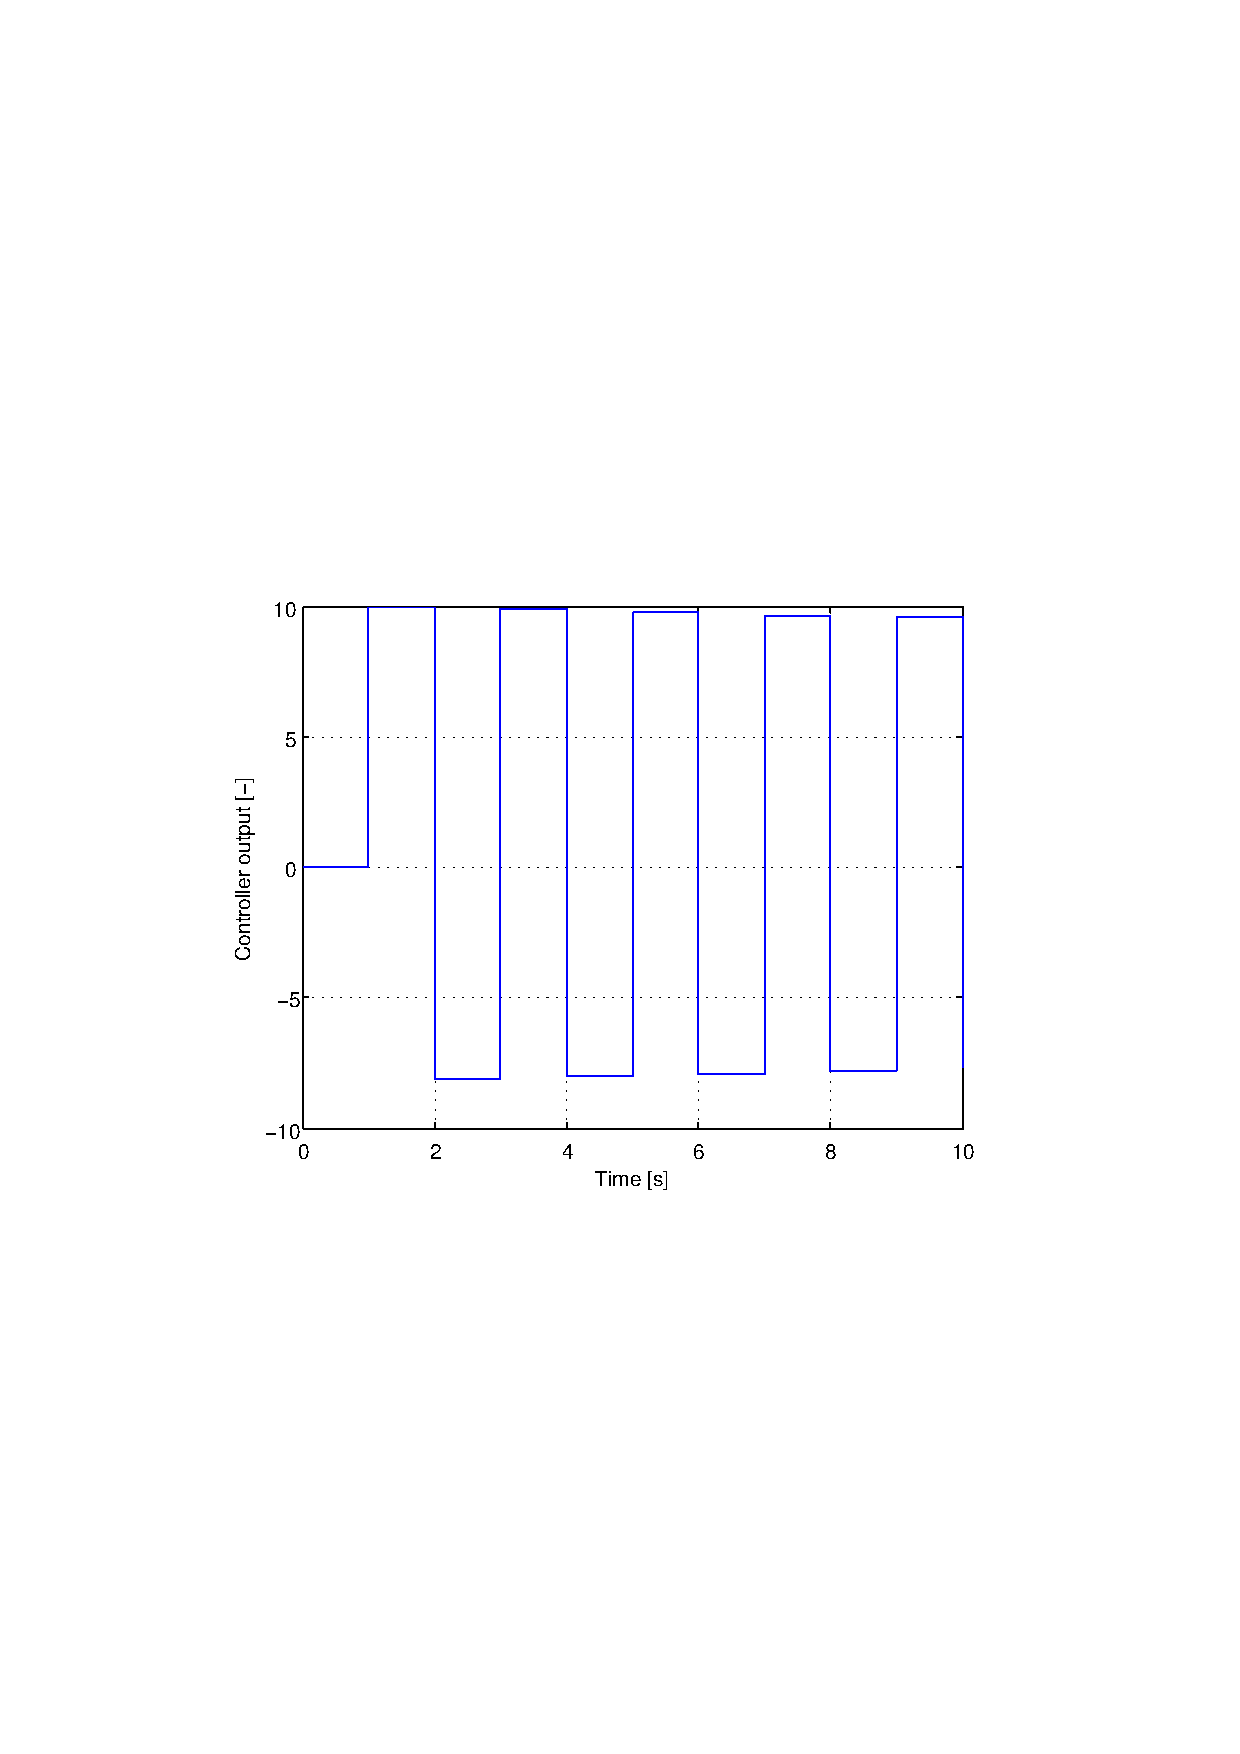
\includegraphics[trim=5cm 9cm 5cm 9cm,width=10cm]{../res/img/d1_1_10u.pdf} 
	\end{center}
	\caption{Odpowiedź obiektu 1-wszego rzędu dla parametrów $k=10$,
	$T_p=1[s]$}
\end{figure}

\newpage

\begin{figure}[!htb]
	\begin{center}
		\includegraphics[trim=5cm 9cm 5cm
		9cm,width=10cm]{../res/img/d1_5_2,165y.pdf}
	\end{center}
	
	\begin{center}
		\includegraphics[trim=5cm 9cm 5cm
		9cm,width=10cm]{../res/img/d1_5_2,165u.pdf}
	\end{center}
	\caption{Odpowiedź obiektu 1-wszego rzędu dla parametrów $k=2,165$,
	$T_p=5[s]$}
\end{figure}

\newpage

\begin{figure}[!htb]
	\begin{center}
		\includegraphics[trim=5cm 9cm 5cm 9cm,width=10cm]{../res/img/d1_10_1,31y.pdf} 
	\end{center}
	
	\begin{center}
		\includegraphics[trim=5cm 9cm 5cm 9cm,width=10cm]{../res/img/d1_10_1,31u.pdf} 
	\end{center}
	\caption{Odpowiedź obiektu 1-wszego rzędu dla parametrów $k=1,31$,
	$T_p=10[s]$}
\end{figure}

\newpage

\subsection{Obiekt trzeciego rzędu}

Poniżej zamieszczam schemat zastępczy układu regulacji cyfrowej obiektu
trzeciego rzędu:
 
\begin{figure}[!htb]
	\begin{center}
		\includegraphics[width=14cm]{../res/img/schd3.png} 
	\end{center}
	\caption{Schemat badanego układu z obiektem inercyjnym trzeciego rzędu}
\end{figure}

Dla tak zestawionego układu wyznaczyliśmy odpowiedzi skokowe i przebiegi
sterowania dla wzmocnienia krytycznego przy poszczególnych okresów próbkowania,
$Tp\in \{0.01, 0.1, 1, 5, 10\}[s]$. W celu wyznaczenia wzmocnienia krytycznego
układu 3-ciego rzędu dla regulacji ciągłej ze schematu usunięty został blok ZOH.
Jak się jednak okazuje wzmocnienie krytyczne dla układu z ekstrapolatorem o
okresie próbkowania równym $T_p=0.01[s]$ jest identyczne jak dla układu bez
ekstrapolatora. Wynika to z tego że zbliżyliśmy się ze sztucznym czasem
próbkowania na tyle do kroku solvera \textsc{Simulink}-a, iż jest on pomijalny.

Poniżej zamieszczone owe odpowiedzi z krótkimi opisami parametrów dla których
zostały ściągnięte.
 
\newpage

\begin{figure}[!htb]
	\begin{center}
		\includegraphics[trim=5cm 9cm 5cm 9cm,width=10cm]{../res/img/d2_c_7,95y.pdf}
	\end{center}
	 
	\begin{center}
		\includegraphics[trim=5cm 9cm 5cm 9cm,width=10cm]{../res/img/d2_c_7,95u.pdf} 
	\end{center}
	\caption{Odpowiedź obiektu 3-ciego rzędu dla parametrów $k=7,95$ bez
	ekstrapolatora}
\end{figure}

\newpage

\begin{figure}[!htb]
	\begin{center}
		\includegraphics[trim=5cm 9cm 5cm 9cm,width=10cm]{../res/img/d2_0,1_7,75y.pdf}
	\end{center}
	
	\begin{center}
		\includegraphics[trim=5cm 9cm 5cm 9cm,width=10cm]{../res/img/d2_0,1_7,75u.pdf} 
	\end{center}
	\caption{Odpowiedź obiektu 3-ciego rzędu dla parametrów $k=7,75$,
	$T_p=0,1[s]$}
\end{figure}

\newpage

\begin{figure}[!htb]
	\begin{center}
		\includegraphics[trim=5cm 9cm 5cm 9cm,width=10cm]{../res/img/d2_1_6,2y.pdf}
	\end{center}
	
	\begin{center}
		\includegraphics[trim=5cm 9cm 5cm 9cm,width=10cm]{../res/img/d2_1_6,2u.pdf} 
	\end{center}
	\caption{Odpowiedź obiektu 3-ciego rzędu dla parametrów $k=6,2$,
	$T_p=1[s]$}
\end{figure}

\newpage

\begin{figure}[!htb]
	\begin{center}
		\includegraphics[trim=5cm 9cm 5cm 9cm,width=10cm]{../res/img/d2_5_3,73y.pdf}
	\end{center}
	
	\begin{center}
		\includegraphics[trim=5cm 9cm 5cm 9cm,width=10cm]{../res/img/d2_5_3,73u.pdf} 
	\end{center}
	\caption{Odpowiedź obiektu 3-ciego rzędu dla parametrów $k=3,73$,
	$T_p=5[s]$}
\end{figure}

\newpage

\begin{figure}[!htb]
	\begin{center}
		\includegraphics[trim=5cm 9cm 5cm 9cm,width=10cm]{../res/img/d2_10_3,15y.pdf}
	\end{center}
	
	\begin{center}
		\includegraphics[trim=5cm 9cm 5cm 9cm,width=10cm]{../res/img/d2_10_3,15u.pdf} 
	\end{center}
	\caption{Odpowiedź obiektu 3-ciego rzędu dla parametrów $k=3,15$,
	$T_p=10[s]$}
\end{figure}

\newpage

\subsection{Wnioski i spostrzeżenia}

Jak widać po wykonanych pomiarach dobór okresu próbkowania ma kluczowy wpływ na
stabilność zamkniętego układu regulacji z regulatorem cyfrowym.

Układ regulacji proporcjonalnej sterujący obiektem inercyjnym rzędu pierwszego,
który zrealizowany fizycznie jest stabilny niezależnie od wzmocnienia regulatora, w
układzie regulacji dyskretnej staje się obiektem niestabilnym dla dużych
wartości wzmocnienia.

Dzieje się tak, ponieważ regulator zbyt rzadko otrzymuje informację o stanie
obiektu, w związku z czym nie jest w stanie wystarczająco szybko zareagować na
nieporządane zmiany sygnału wyjściowego.

Jest to szczególnie widoczne dla niepoprawnie dobranej
częstotliwości próbkowania sygnału. Można zauważyć prawidłowość - zmiana okresu
próbkowania o rząd, powodóję również zmianę rzędu wzmocnienia które wprowadza
układ na granicę stabilności.

\newpage

\section{Analiza serwomechanizmu przekaźnikowego z wykorzystaniem
 płaszczyzny fazowej}

\subsection{Cel ćwiczenia}

Celem ćwiczenia jest zapoznanie się z zastosowaniem metody płaszczyzny fazowej do analizy nieliniowych
układów regulacji na przykładzie serwomechanizmu przekaźnikowego. Podczas ćwiczenia zbadany zostanie
wpływ parametrów zarówno przekaźnika, jak i obiektu na przebieg trajektorii fazowych serwomechanizmu
przy zerowym wymuszeniu i starcie z niezerowych warunków początkowych. Należy zbadać przebieg
trajektorii fazowych dla układu regulacji złożonego z obiektu o transmitancji:

\begin{equation*}
	G(s)=\frac{K}{s(Ts+1)}
\end{equation*}

oraz regulatora III położeniowego z histerezą.

\begin{figure}[!htb]
	\begin{center}
		\includegraphics[width=14cm]{../res/img/schs1.png} 
	\end{center}
	\caption{Schemat badanego układu regulacji serwomechanizmu}
\end{figure}

\newpage

\subsection{Serwomechanizm bez opóźnienia}

Dla przypadku $T=0[s]$ serwomechanizm jest obiektem podwójnie całkującym. Jest
to obiekt trudny do sterowania, ponieważ nawet po zaniku wymuszenia sygnał
wyjściowy będzie narastał do nieskończoności. Jest to więc obiekt astatyczny.

\begin{figure}[!htb]
	\begin{center}
		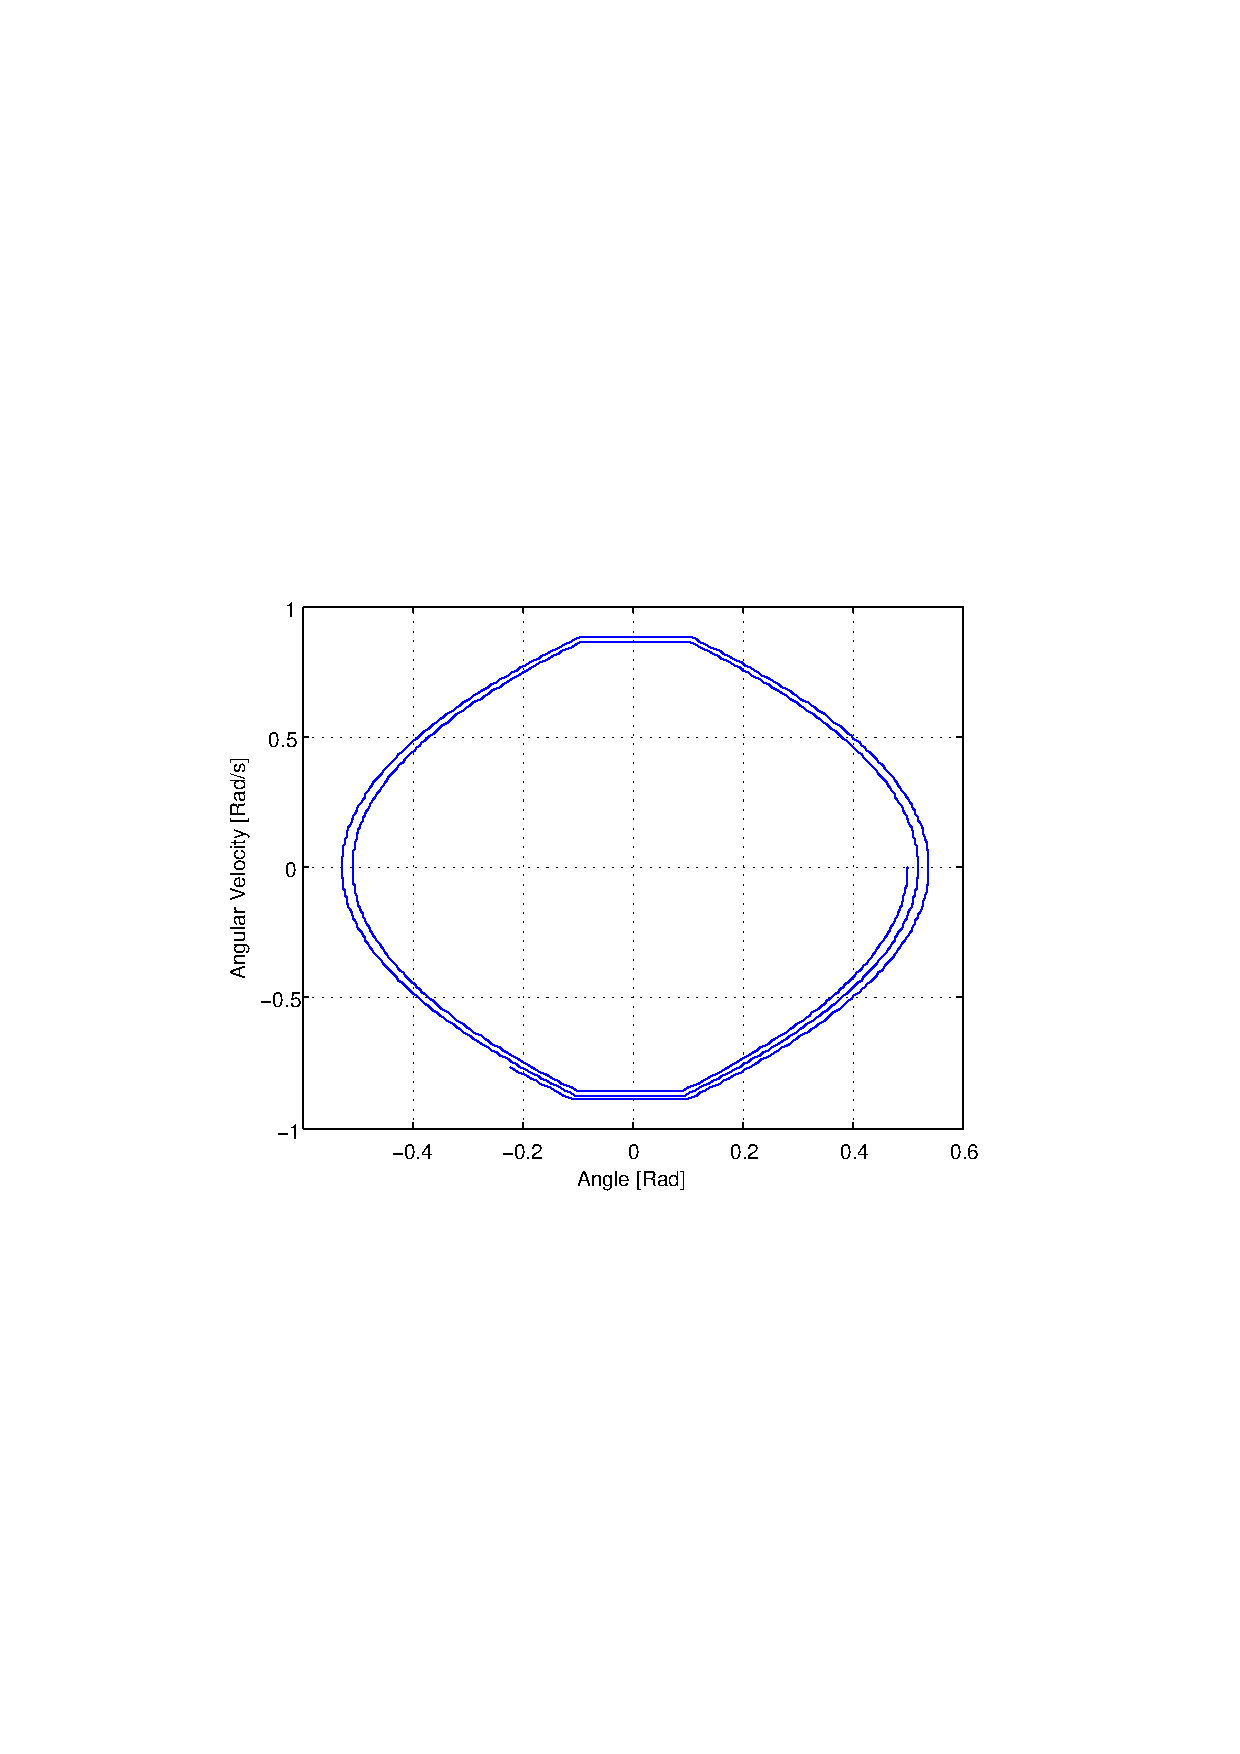
\includegraphics[trim=5cm 9cm 5cm 9cm,width=9cm]{../res/img/s1_T0_N0,1_h0_K1_e1-0_e0-0,5p.pdf}
	\end{center}
	
	\begin{center}
		\includegraphics[trim=5cm 9cm 5cm 9cm,width=9cm]{../res/img/s1_T0_N0,1_h0_K1_e1-0_e0-0,5r.pdf} 
	\end{center}
	\caption{Charakterystyka fazowa, oraz odpowiedź obiektu bez inercji dla
	nastaw $N=0.1$, $h=0$, $K=1$, $e_1=0$, $e_0=0.5$}
\end{figure}

\newpage

\begin{figure}[!htb]
	\begin{center}
		\includegraphics[trim=5cm 9cm 5cm
		9cm,width=9cm]{../res/img/s1_T0_N0,1_h0,05_K1_e1-0_e0-0,5p.pdf}
	\end{center}
	
	\begin{center}
		\includegraphics[trim=5cm 9cm 5cm
		9cm,width=9cm]{../res/img/s1_T0_N0,1_h0,05_K1_e1-0_e0-0,5r.pdf}
	\end{center}
	\caption{Charakterystyka fazowa, oraz odpowiedź obiektu bez inercji dla
	nastaw $N=0.1$, $h=0.05$, $K=1$, $e_1=0$, $e_0=0.5$}
\end{figure}

Jak widać dodanie histerezy pogorszyło tylko wynik regulacji, który i bez
histerezy był fatalny, ponieważ układ był niestabilny. O stabilności układu
można poza odpowiedzią skokową również wywnioskować z charakterystyki fazowej.
Jeśli obiekt jest niestabilny charakterystyka niejako ``rozwija się''. Układ
jest stabilny, gdy charakterystyka znajduje punkt w którym się zatrzymuje. Musi
być to punkt na osi poziomej, ponieważ wartości pionowe na charakterystyce
fazowej oznaczają w naszym wypadku prędkość kątową serwomechanizmu.

\subsection{Serwomechanizm z opóźnieniem}

Dla przypadku $T>0[s]$ serwomechanizm jest obiektem całkującym z inercją.
Jest to obiekt dużo bardziej podatny na sterowanie niż w przypadku braku 
inercji. Nie jest to właściwie spowodowane obecnością inercji, lecz tym iż
obiekt inercyjny po zaniku sterowania wraca do położenia równowagi, więc również
odpowiedź całego obiektu będzie ograniczona po zaniku wymuszenia.

\begin{figure}[!htb]
	\begin{center}
		\includegraphics[trim=5cm 9cm 5cm 9cm,width=9cm]{../res/img/s1_T1_N0,1_h0_K1_e1-0_e0-0,5p.pdf}
	\end{center}
	
	\begin{center}
		\includegraphics[trim=5cm 9cm 5cm 9cm,width=9cm]{../res/img/s1_T1_N0,1_h0_K1_e1-0_e0-0,5r.pdf} 
	\end{center}
	\caption{Charakterystyka fazowa, oraz odpowiedź obiektu z inercją $T=1$ dla
	nastaw $N=0.1$, $h=0$, $K=1$, $e_1=0$, $e_0=0.5$}
\end{figure}

\newpage

\begin{figure}[!htb]
	\begin{center}
		\includegraphics[trim=5cm 9cm 5cm
		9cm,width=9cm]{../res/img/s1_T1_N0,1_h0,04_K1_e1-0_e0-0,5p.pdf}
	\end{center}
	
	\begin{center}
		\includegraphics[trim=5cm 9cm 5cm
		9cm,width=9cm]{../res/img/s1_T1_N0,1_h0,04_K1_e1-0_e0-0,5r.pdf}
	\end{center}
	\caption{Charakterystyka fazowa, oraz odpowiedź obiektu z inercją $T=1$ dla
	nastaw $N=0.1$, $h=0.04$, $K=1$, $e_1=0$, $e_0=0.5$}
\end{figure}

Dla układu regulatora bez histerezy udaje nam się trafić w jego strefę
nieczułości z odpowiedzią obiektu dlatego też stabilizuje się on całkowicie już
po pierwszej oscylacji. Nie jest to jednak stabilny stan. Drobne zakłócenie może
wybić obiekt z równowagi.

Wyraźnie widać na przykładzie układu z histerezą, że ta zmiana parametru
pozwoliła wprowadzić układ w stan normalnej pracy oscylacje wielkości wyjściowej
wachają się w granicach strefy nieczułości plus histereza plus wielkość zależna
od bezwładności obiektu, którą trudno ocenić.

\newpage

\subsection{Wnioski i spostrzeżenia}

Wykres fazowy odpowiedzi układu jest ściśle związany z jego odpowiedzią czasową.
Jedna z osi opisuje szybkość zmian sygnału wyjściowego, natomiast druga jego
wartość. Po przebiegu wykresu fazowego możemy w przybliżony sposób (tracimy
informację o czasie) oszacować kształt odpowiedzi czasowej, np. wiemy że gdy
wykres fazowy zatacza figury wokół środka układu współżędnych na wyjściu obiektu
występują oscylacje.

\end{document}